\subsection{Plant Scaling}
\label{sec:plantscale}

Plant scaling is a rather important section as it dictates the flowrates and storage requirements the plant has to adhere to, in order to satisfy consumer demand for the first design iteration.

The plant simulation was used with demand and wind data fed into a MATLAB program, which followed this process flow:
\begin{enumerate}
    \item Program found the net energy in the system by subtracting load from wind generation.
    \item Program assumed the net energy on the grid was zero, and all shortfalls and surplus were satisfied by the plant.
    \item Program logged total energy generated, and total energy fed into plant for a year.
\end{enumerate}

A flowsheet was then generated by using typical values from literature, with the assumption the gas turbine has a duty cycle of 5\% of all generation.
The material balance for the first design iteration was produced in Figure \ref{flowsheettbl}.
These data were used to scale other components and to demonstrate that with approximate efficiency values from literature that this is a feasible project.
Components were scaled by a safety factor applied to their predicted maximum use, 1.3 for the Gas Turbine, 1.2 for the SOFC, and 1.5 for the Electrolyser, with their respective powers in Table \ref{tbl:powercomp}.
A rather startling conclusion from this analysis is that the ESS stores far less energy than was originally expected.
The wind speeds in Maui are sufficiently high all-year-round to satisfy the bulk of consumer demand.

\begin{figure}[tbh]
    \centering
    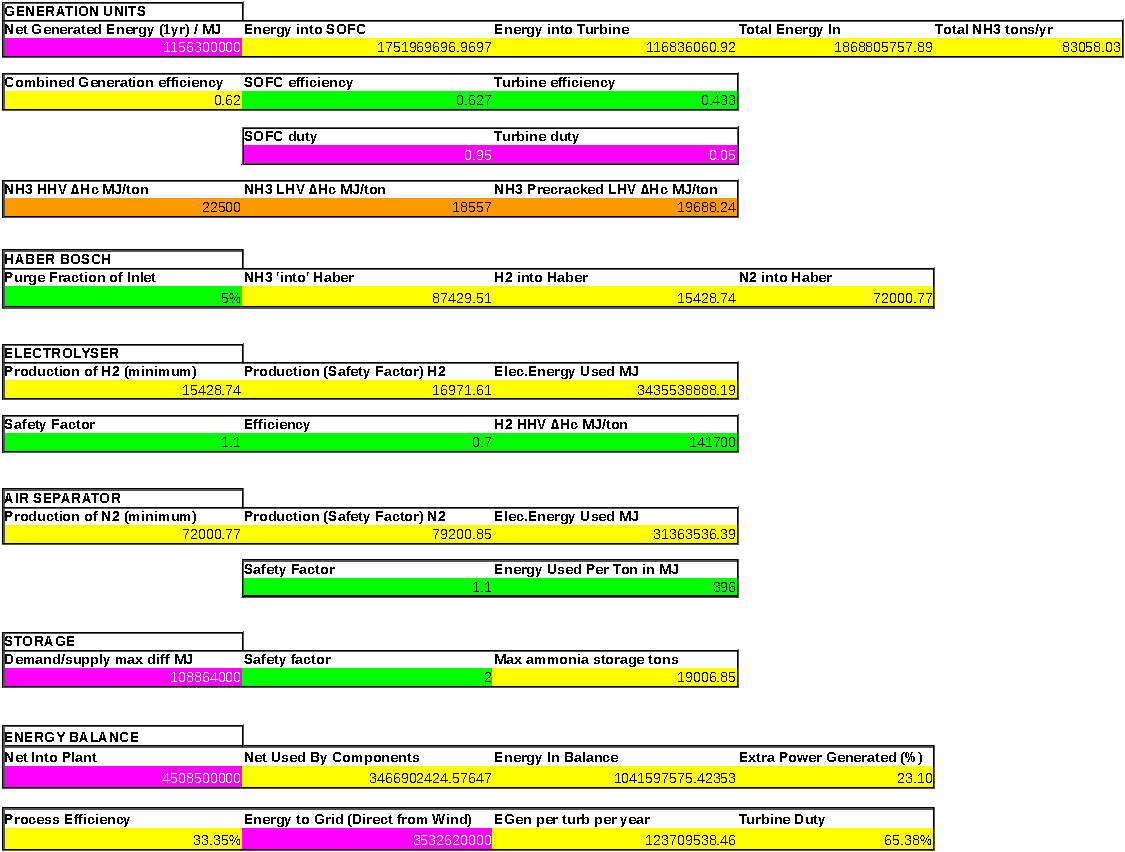
\includegraphics[scale=0.9]{images/flowtable.pdf}
    \caption{An approximate material balance flowsheet using efficiency factors from all components, demand and wind data.}
    \label{flowsheettbl}
\end{figure}

These data allowed for an idea of the plant's scale, and were used to find more detailed component parameters for the plant's dynamic simulation. 